\documentclass[MAIN.tex]{subfiles} 
\begin{document} 
%======================================================================================= %
\begin{frame}[fragile]
	\frametitle{The Geometric Probability Distribution}
	\large
	\begin{itemize}
\item	Used for binary data (1 or 0; success or failure, etc). 
\item In a sequence of trials, the trial yielding the first success (all previous trials ending in failure) has a geometric distribution. 
\item The assumption required is that separate trials are independent and the probability of success p is the same in every trial. 
\item The probability of failure in each trial is $1 - p$.
	\end{itemize}

\end{frame}
%======================================================================================= %
\begin{frame}[fragile]
	\frametitle{The Geometric Probability Distribution}
%	The variable X counts the number of \textbf{\textit{failures}} before the first \textbf{\textit{success}}. In other words, X = 0 if success occurs on the 1st trial. X = 1 means that the 1st trial ended in failure and success occurred in the 2nd trial. X = 2 means that the 1st and 2nd trial ended in failure and that success occurred in the 3rd trial. And so on. $Pr[X]$ is calculated as
\begin{framed}
	\begin{verbatim}
	# p is the probability of success
	dgeom(X, prob = p)            
	# log of the probability instead
	dgeom(X, prob = p, log=TRUE)  
	\end{verbatim}
\end{framed}
\end{frame}
%======================================================================================= %
\begin{frame}[fragile]
	\frametitle{The Geometric Probability Distribution}
	
	\begin{figure}
		\centering
		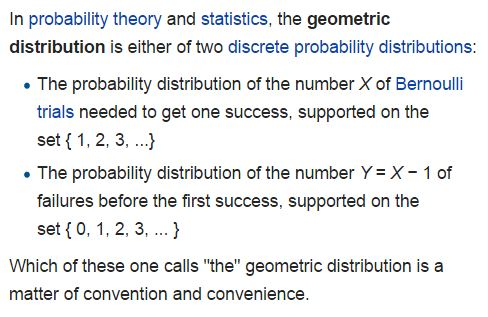
\includegraphics[width=1.05\linewidth]{images/geometric}
		
	\end{figure}
	
\end{frame}
%======================================================================================= %
\begin{frame}[fragile]
	\frametitle{The Geometric Probability Distribution}
	
	\begin{figure}
		\centering
		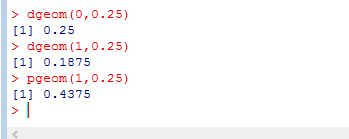
\includegraphics[width=1.05\linewidth]{images/geometric2}
		
	\end{figure}
\end{frame}
%===================================================================== %
\end{document}


